\documentclass[12pt,a4paper]{article}
\usepackage{amsmath}
\usepackage{amsfonts}
\usepackage{amssymb}
\usepackage{graphicx}
\usepackage{secdot}
\usepackage[left=2cm,right=2cm,top=2cm,bottom=2cm]{geometry}

\author{ Shibayan Biswas, AE21B109,\\ Department of Aerospace Engineering,\\ IIT Madras\\[3ex] Instructor:\\ \large Professor Dr. Vadlamani Nagabhushana Rao}

\title{Experiment- 1}

\date{November 16, 2022}

\begin{document}

\maketitle
\hline
\section{Aim:}
To observe the behaviour of standing waves and the variations in those standing waves by using the Ruben's Tube.
\section{Introduction:}
A Rubens tube, also known as a standing wave flame tube, or simply flame tube, is a physics apparatus for demonstrating acoustic standing waves in a tube.\\
\begin{figure}[!ht]
	\begin{center}
			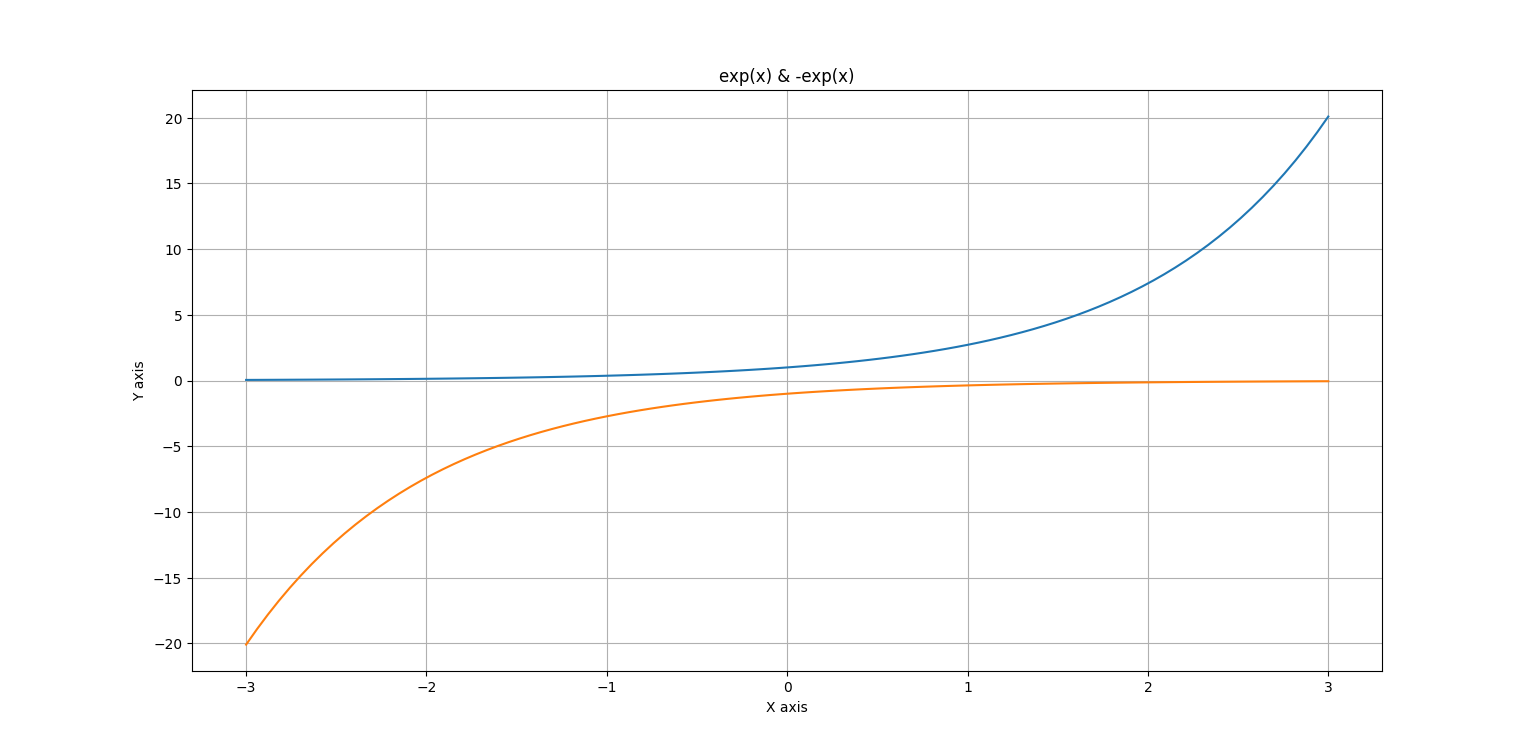
\includegraphics[scale=0.5]{Figure_1.jpg}
	\end{center}
	\caption{Setup for Ruben's Tube Experiment}
\end{figure}\\
\noindent
A length of pipe is perforated along the top and sealed at both ends - one seal is attached to a small speaker or frequency generator, the other to a supply of a flammable gas. The pipe is filled with the gas, and the gas leaking from the perforations is lit. If a suitable constant frequency is used, a standing wave can form within the tube. When the speaker is turned on, the standing wave will create points with oscillating (higher and lower) pressure and points with constant pressure (pressure nodes) along the tube. Where there is oscillating pressure due to the sound waves, less gas will escape from the perforations in the tube, and the flames will be lower at those points. At the pressure nodes, the flames are higher. At the end of the tube gas molecule velocity is zero and oscillating pressure is maximal, thus low flames are observed. This height of flame is increased if the amplitude of the sound is increased as the total energy being fed into the pipe increases. It is possible to determine the wavelength from the flame minimum and maximum by simply measuring with a ruler.\\ 
\\Consider a standing wave in a pipe of length L. The air inside the pipe serves as the medium for longitudinal sound waves traveling to the right or left through the pipe. the waves traveling through
the air in the pipe vary in terms of their pressure and longitudinal displacement along the direction of wave motion. The wave propagates by alternately compressing and expanding air in segments of the pipe, which displaces the air slightly from its rest position and transfers energy to neighboring segments through the forces exerted by the alternating high and low air pressures.
\section{Apparatus:}
The figure given below shows the Ruben's Tube and its components:
\begin{itemize}
\item \textbf{Metal Tube:} We have a metal pipe with one end sealed with a scrap iron plate and the other end open to sound waves. It consists of a row of evenly spaced holes through which we see the flames.
\item \textbf{Gas cylinder:} We have a gas cylinder that releases fuel gas into the pipe. The gas inlet is close to the sealed end. LPG here, is the only gas injected into the pipe without an oxidising agent. Hence, it burns with a yellow flame indicative of incomplete combustion.
\\The flame used is a diffusion flame. In combustion, a diffusion flame is a flame in which the oxidizer and fuel are separated before burning.
\item \textbf{Speaker:} Right next to the open end we have a speaker that produces sound waves of selected frequencies and volumes.
\end{itemize}
\begin{figure}[!ht]
	\begin{center}
		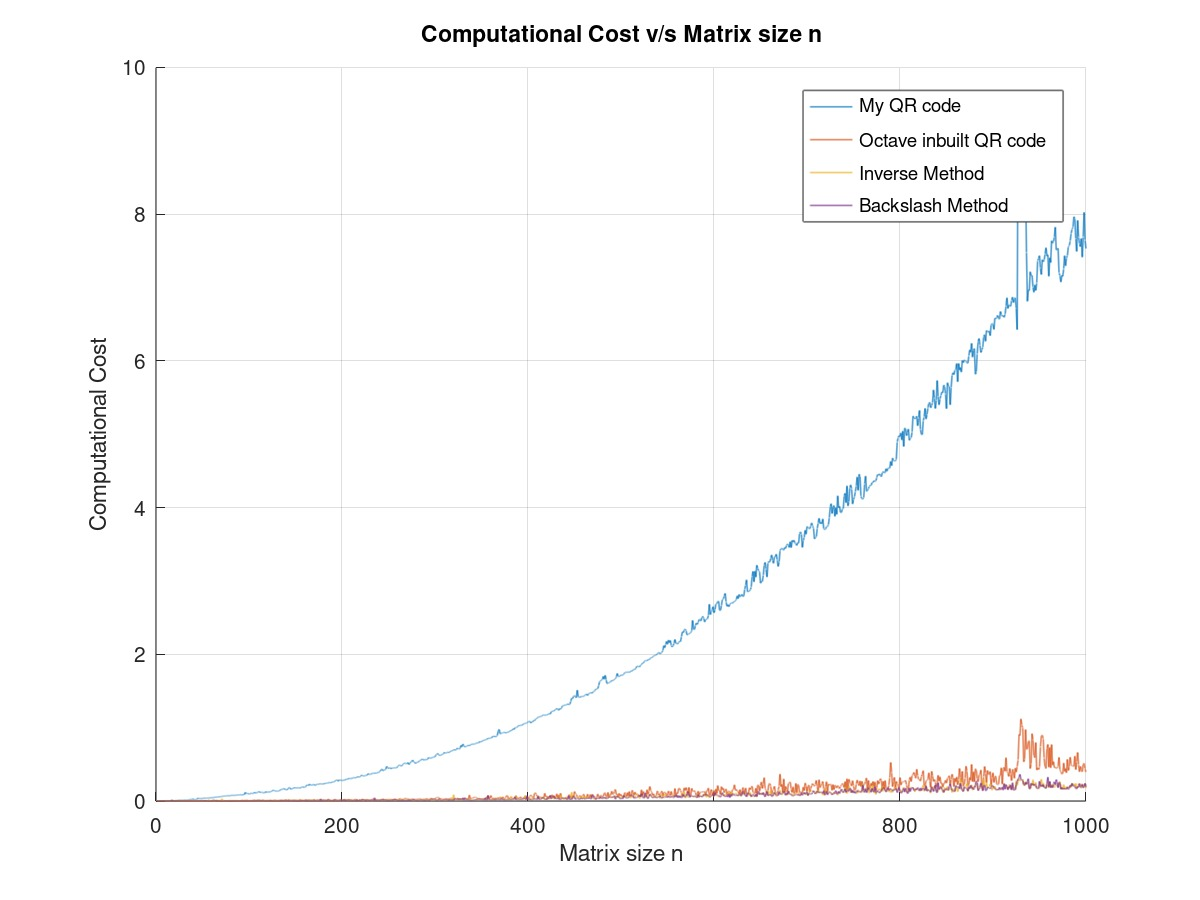
\includegraphics[scale=0.9]{Figure_2.jpeg}
	\end{center}
	\caption{Apparatus for Ruben's Tube Experiment}
\end{figure}
\clearpage
\section{Theory:}
Ruben’s Tube consists of a large diameter (normally metal tube) with a series of holes drilled in the top. A loudspeaker is attached to one end, and a flammable gas supply to the other, and the gas coming out of the holes is lit. When the loudspeaker vibrates it sends a series of waves of gas down the tube at the
speed of sound, these then reflect off the far end of the tube, so there are two sets of waves moving through the tube in opposite directions. when the length of the tube is a multiple of half the wavelength the two waves add together to form what is known as a standing wave. In some places the two waves add together forming extra large changes in pressure (anti-nodes) and in other areas they cancel each other out so the pressure is constant (nodes). When the gas is first lit the flames will be about the same height due to the constant pressure,but once the sound is transmitted through the tube the flames begin to vary in height because of pressure change.The Rubens’ Tube illustrates a standing wave that represents the sound that is being played.\\
\begin{figure}[!ht]
	\begin{center}
		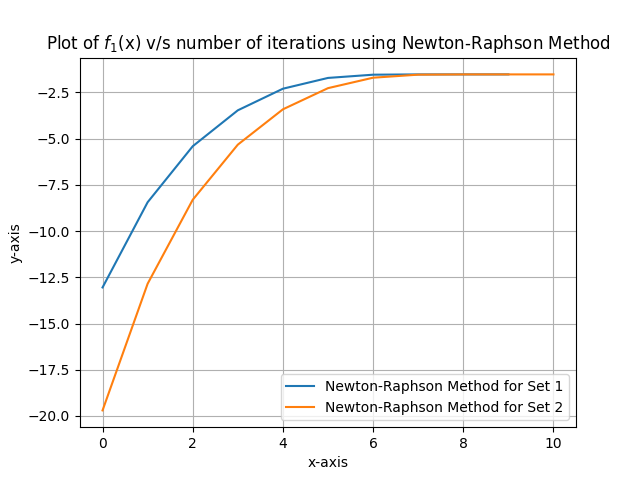
\includegraphics[scale=0.35]{Figure_3.jpg}
	\end{center}
	\caption{Formation of standing waves inside Ruben’s Tube}
\end{figure}
\subsection{Bernoulli's Principle:}
The working of Rubens tube is based on the Bernoulli’s principle which states that:
\begin{equation}
    \text{P} + \frac{1}{2}\text{\rho$v^2$} + \text{$\rho gh$} = \text{constant}
\end{equation}
On applying Bernoulli's’s theorem inside and outside the Ruben's’ Tube , we get,
The time-averaged mass flow rate of the gas is proportional to the square root of the pressure difference between the inside(i.e the pressure of gas) and outside of the tube(i.e atmospheric pressure).
\begin{equation}
    \text{v} \propto \text{$\sqrt{P_T - P_{atm}}$}
\end{equation}
where $v$ is the velocity of gas with which it comes out of the tube, $P_T$ is the gas pressure inside the tube and $P_{atm}$ is the atmospheric pressure.
\clearpage
\begin{figure}[!ht]
	\begin{center}
		\framebox{
			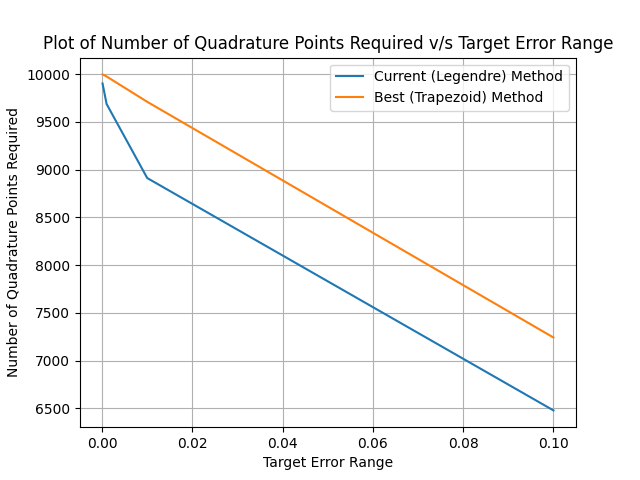
\includegraphics[scale=0.8]{Figure_4.png}
		}
	\end{center}
	\caption{Standing Waves inside Ruben’s Tube}
\end{figure}
\noindent
The pink wave is the forward traveling wave, the orange wave is reflected wave and the yellow wave is the standing wave. The maxima in the flame occurs at the pressure nodes while the minima occurs at pressure anti-node.The increase outward flow rate when the pressure is at it’s maxima is less than the decrease in outward flow when there is a pressure minima this is because flow rate is proportional to square root of pressure difference and not just pressure
difference. So at anti-nodes there is a net decrease in flow rate which creates a minima in the flame.\\
\\The yellow wave represents the pressure standing wave and the blue line represents the change in flow rate.As we can see the decrease in flow rate is more then increase in flow rate at anti-nodes so minima in flame occurs at anti-nodes and maxima occurs at nodes. As the sound become louder and louder the flame maxima and minima shift their position.After a point the minima starts to appear at node and maxima at anti-node.This is because as the amplitude of the sound increases, the minimum pressure in the pipe drops below the ambient pressure.\\
\begin{figure}[!ht]
	\begin{center}
		\framebox{
			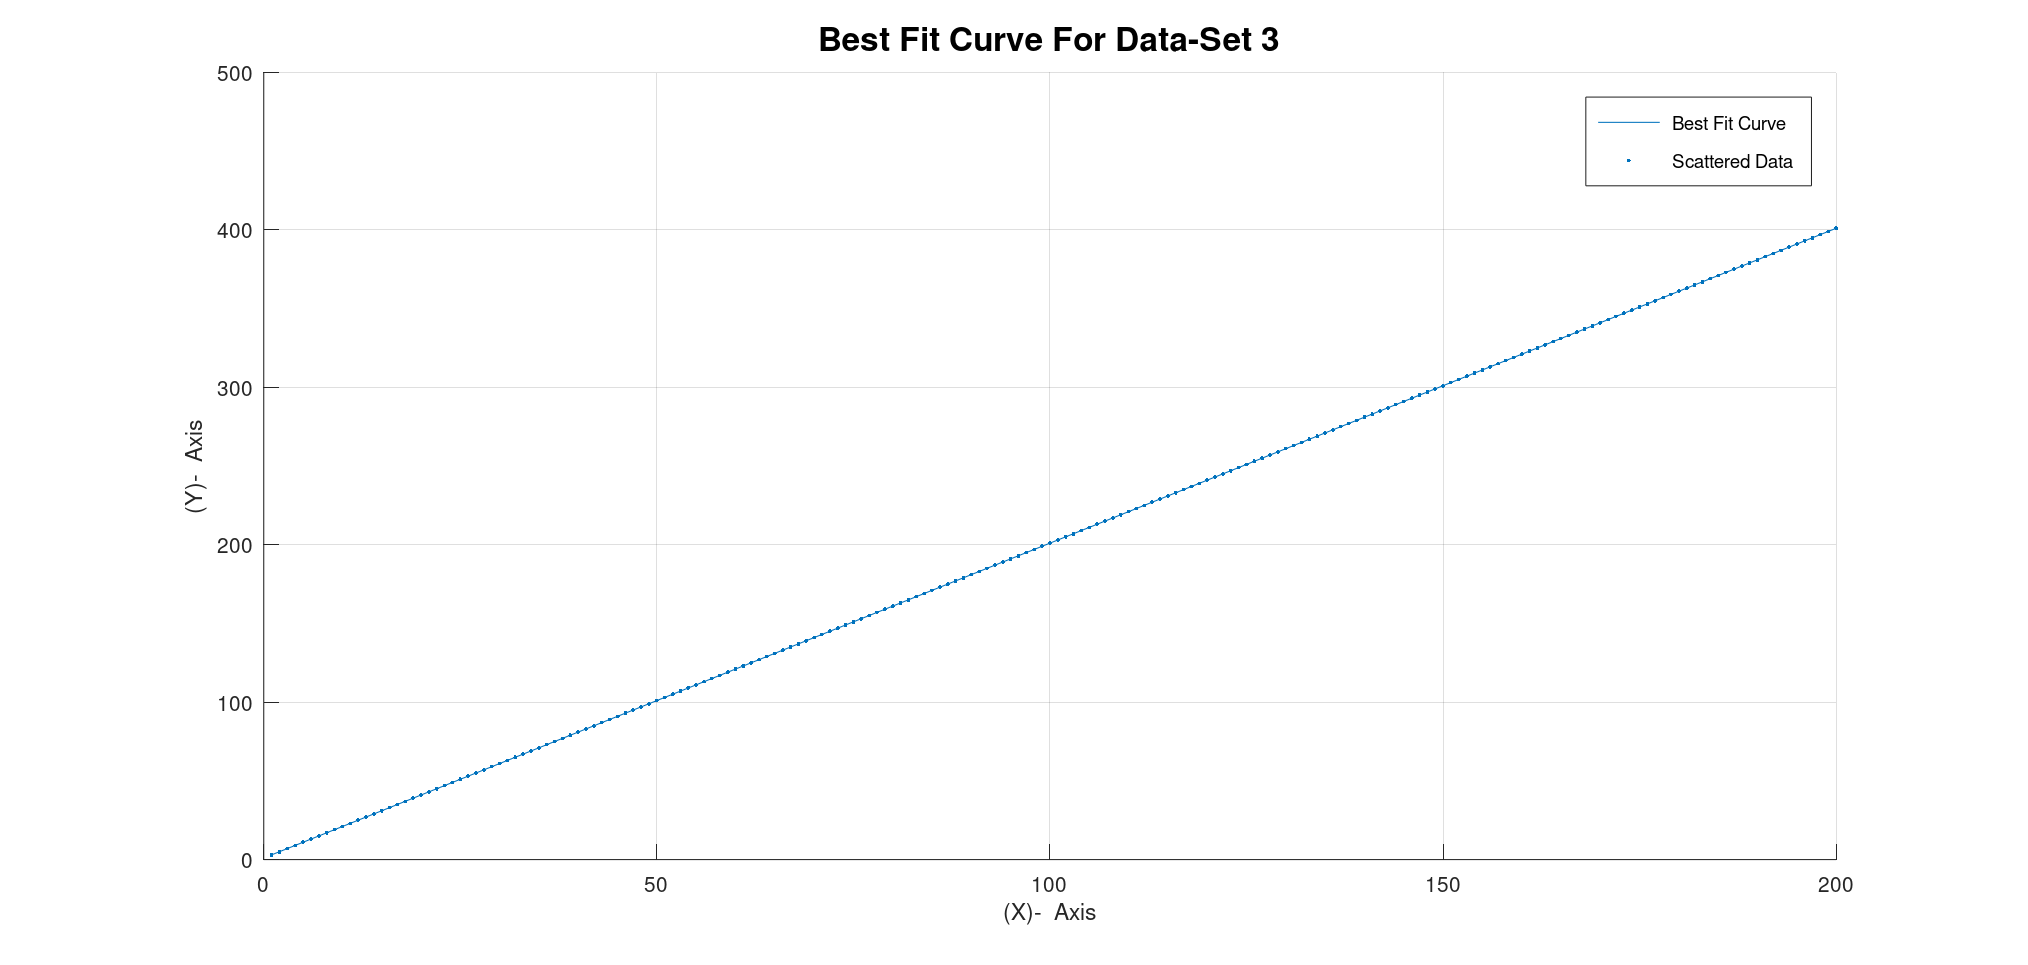
\includegraphics[scale=0.8]{Figure_5.png}
		}
	\end{center}
\end{figure}
\clearpage
\noindent
When the pressure is highest, a significant amount of gas is expelled through the hole. This fuel hits the existing flame, igniting and generating heat causing the gases to rise further and expel the combustion gases further from the hole. Once the pressure drops below ambient pressure, gas is drawn in, into the pipe. This gas consists of a mixture of unburned fuel gas + air. When pressure in tube falls below ambient pressure, the Rubens’ Tube cannot recapture and inhale the exact same jet that it exhaled thus at anti-nodes there is hysteresis where at
maximum pressure inside tube the flame becomes bigger and is only slightly hindered by negative pressure.
\subsection{Speed of Sound:}
If we denote the frequency of sound as $f$, its speed in the medium as $v$ and wavelength as $\lambda$, then these three parameters are linked together by the equation:\\
\begin{equation}
    \text{$v$} = \text{$f$} \text{$\lambda$}
\end{equation}
\begin{figure}[!ht]
	\begin{center}
		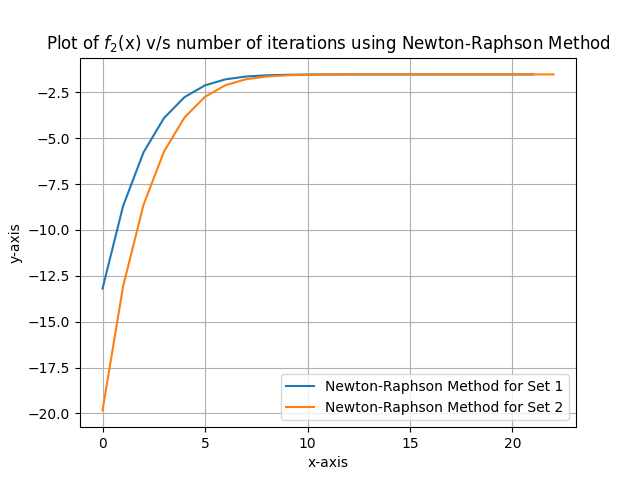
\includegraphics[scale=1.3]{Figure_6.jpeg}
	\end{center}
\end{figure}
\section{Mechanism:}
Ruben’s Tube is a classic physical device to show that sound waves mainly compress waves and give a visual display of waves standing by a flame.\\
\\In 1905, the German scientist Heinrich Rubens invented the original device four meters long from a tube with 200 holes of equal diameters distributed steadily along its length. The Tube ends were closed, and flammable gas pumped into it, and the gas escaped from the holes and then lit up to form flames. A loudspeaker was connected to one end of the device, and the sound was played at frequencies at which the flame heights changed, illustrating the pressure
differences created inside the tube due to the sound waves.\\
\\This apparatus is based on Bernoulli’s principle. The time-averaged mass flow rate of the gas is proportional to the square root of the pressure difference between the inside and outside of the tube. A standing wave is formed with a constant frequency when the leaking gas from perforations is lit. If the speaker is turned on, nodes and anti-nodes are formed in the tube. Generally, the maximum height of the flame can occur at nodes or anti-nodes. But, the height of the flame varies with the change in operation of the tube. It usually has two modes of operation- ”normal” and ”reversal”. Under normal operation, the pressure nodes have tall, yellow flames and the pressure anti-nodes have short, blue flames.\\
\\ This shows that the time-averaged mass flow rate is greatest at the holes corresponding to pressure nodes. Thus, the flame maxima occurs at the pressure nodes. However, at high sound intensities of 140-150 dB, the time-averaged pressure variation due to non-linearity causes the operation to change.\\
\\As the gas static pressure was reduced or acoustic levels increased, we observe a “reversal” in flame height - flames are greater in height at the anti-nodes than at the nodes. It is also observed that an intake of unburned gas and possibly air takes place at the anti-nodes, referred to as “gulping.” Gulping may be caused by the acoustic oscillations being greater in amplitude
that the static pressure flow, which results in a temporarily negative/inward mass flow rate during the rarefacting wave near the anti-nodes. The following steps are followed to perform the experiment:\\
\begin{itemize}
\item We open the gas cylinder valve and propane flows into the pipe. The pressure inside the tube is raised from atmospheric pressure by amount $\Delta P$.
\item The gas flows out of the holes in the pipe as indicated by the flames. Making necessary assumptions about the flow, and using flame height as an indicator of the velocity of the gas from a particular hole, we can say that:
\begin{equation}
    \text{v} = \sqrt{\frac{\text{$2 \Delta P$}}{\text{$\rho$}}}
\end{equation}
\item We produce a sound wave through the speaker, pressure waves travel through the tube and reflect from the sealed end. The propagating and reflected waves superimpose and form standing waves with nodes and anti-nodes that are reflected in the flame pattern.
\end{itemize}
\section{Observations:}
When the gas is ignited, flames form all along the tiny holes on the side of the tube. When the speaker is turned on, sound waves travel through the propane inside the tube.waves of flame seem to be created and their wavelength changes with the frequency (pitch) of the sound being fed in. The basis for this effect is resonances in the gas in the tube. When the loudspeaker vibrates it sends a series of waves of air down the tube at the speed of sound, these then reflect off the far end of the tube, so there are two sets of waves moving through the tube in opposite directions.\\
\\For most wavelengths this does not produce a very interesting effect, but
when the length of the tube is a multiple of half the wavelength the two waves
add together to form what is known as a standing wave. In some places the
two waves add together forming extra large changes in pressure (anti-nodes)
and in other areas they cancel each other out so the pressure is constant
(nodes).\\
\clearpage
\noindent
We can measure the distance between peaks of the flames. This is the wavelength of the standing wave $\lambda$. We know that the frequency of the sound is $f$ . Hence, we can calculate the speed of the sound wave by using the equation:
\begin{equation}
    \text{$v$} = \text{$f$} \text{$\lambda$}
\end{equation}
When we increase the volume of the sound, the height of the waves increases. Hence, by using the height to obtain the velocity of the peaks of the waves, we can find the maximum value of $\Delta P$. This can then be used to calculate the volume of the sound in decibel by the help of the equation given below:
\begin{equation}
    \text{Loudness ($db$)} = \text{20 $ln$}(\frac{\Delta P}{P_{ref}})
\end{equation}
where, 
\begin{itemize}
\item \textbf{$\Delta P$:} Root Mean Squared value of the pressure of the sound wave .
\item \textbf{$P_{ref}$:} Reference Pressure for humans. Usually it's value is considered as 20 \times $10^{-6}$ Pa .
\end{itemize}
\begin{figure}[!ht]
	\begin{center}
		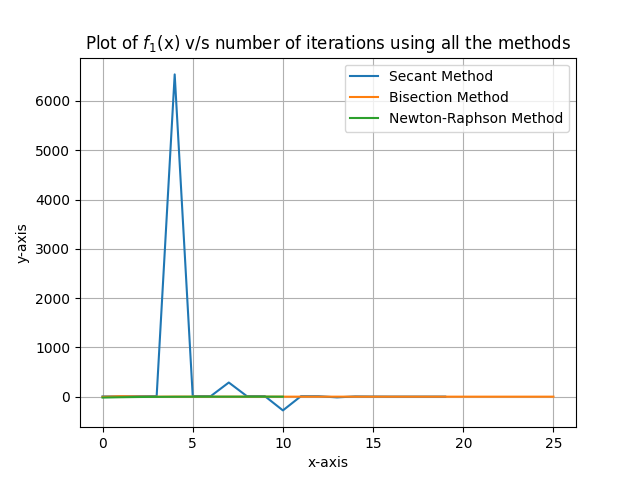
\includegraphics[scale=0.35]{Figure_7.jpg}
	\end{center}
	\caption{Standing waves in Ruben’s Tube}
\end{figure}
\section{Applications:}
The device is now used only as an experimental demonstration of acoustic standing waves in labs. Its use as a scientific instrument to study wave-forms is obsolete now because an oscilloscope serves the purpose with greater accuracy and is more convenient to set up.\\
\\Many musicians and bands make the flames dance to their music for giving a unique audio-visual treat to their audience. Instead of a pipe, some use a cuboid that offers a larger surface area for the holes. This arrangement, known as Pyro Board is an improvisation of the classical structure of the tube and gives a 2D effect of the flames.\\
\\Although the device has only antique value now, it is one of those rare inventions of Physics which allows learners to grip core concepts of standing waves in a visually stimulating way by making the flames dance to the rhythm of sound. In that way, even in this age of digital oscillators, Ruben’s Tube is difficult to beat.
\begin{figure}[!ht]
	\begin{center}
		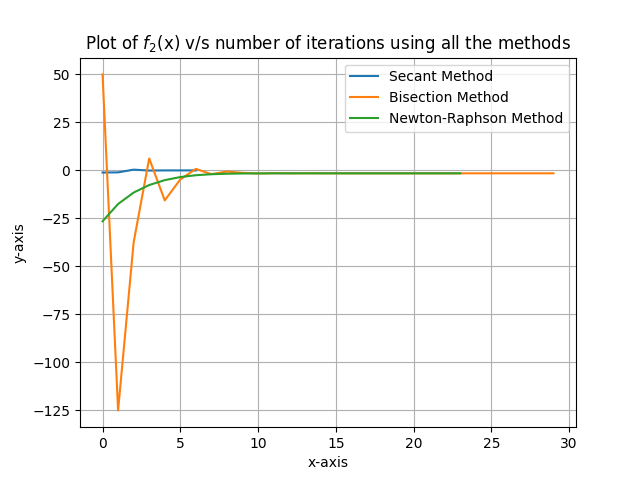
\includegraphics[scale=0.4]{Figure_8.jpeg}
	\end{center}
	\caption{Pyro Board- Application of Ruben's Tube}
\end{figure}
\section{Conclusion:}
From the following experiment I conclude that sound waves are pressure waves. As sound waves propagate through a medium, the compressions and rarefactions create regions of high and low pressure respectively. This pressure differences were visualized as differences in flame height in the Ruben’s Tube. The mass flow rate of the gas is solely influenced by the pressure difference, thus leading to different flame heights.
\section{Precautions:}
\begin{itemize}
\item The tube uses inflammable gas like natural gas or propane as the medium, increasing its potential risk of explosion.
\item The gas supply to the tube should be properly adjusted so that the flames do not reach
large heights.
\item The lab or room where the device is kept is supposed to be very well ventilated to
prevent any accumulation of flammable gas.
\item The frequency or volume of the signal generator is to be adjusted very slowly. Abrupt
changes might cause unexpected changes in the flame height.
\end{itemize}
\end{document}
